%  ---------------------------------------------------------------  %
%            Speech Signal Processing Toolkit (SPTK)                %
%                      SPTK Working Group                           %
%                                                                   %
%                  Department of Computer Science                   %
%                  Nagoya Institute of Technology                   %
%                               and                                 %
%   Interdisciplinary Graduate School of Science and Engineering    %
%                  Tokyo Institute of Technology                    %
%                                                                   %
%                     Copyright (c) 1984-2007                       %
%                       All Rights Reserved.                        %
%                                                                   %
%  Permission is hereby granted, free of charge, to use and         %
%  distribute this software and its documentation without           %
%  restriction, including without limitation the rights to use,     %
%  copy, modify, merge, publish, distribute, sublicense, and/or     %
%  sell copies of this work, and to permit persons to whom this     %
%  work is furnished to do so, subject to the following conditions: %
%                                                                   %
%    1. The source code must retain the above copyright notice,     %
%       this list of conditions and the following disclaimer.       %
%                                                                   %
%    2. Any modifications to the source code must be clearly        %
%       marked as such.                                             %
%                                                                   %
%    3. Redistributions in binary form must reproduce the above     %
%       copyright notice, this list of conditions and the           %
%       following disclaimer in the documentation and/or other      %
%       materials provided with the distribution.  Otherwise, one   %
%       must contact the SPTK working group.                        %
%                                                                   %
%  NAGOYA INSTITUTE OF TECHNOLOGY, TOKYO INSTITUTE OF TECHNOLOGY,   %
%  SPTK WORKING GROUP, AND THE CONTRIBUTORS TO THIS WORK DISCLAIM   %
%  ALL WARRANTIES WITH REGARD TO THIS SOFTWARE, INCLUDING ALL       %
%  IMPLIED WARRANTIES OF MERCHANTABILITY AND FITNESS, IN NO EVENT   %
%  SHALL NAGOYA INSTITUTE OF TECHNOLOGY, TOKYO INSTITUTE OF         %
%  TECHNOLOGY, SPTK WORKING GROUP, NOR THE CONTRIBUTORS BE LIABLE   %
%  FOR ANY SPECIAL, INDIRECT OR CONSEQUENTIAL DAMAGES OR ANY        %
%  DAMAGES WHATSOEVER RESULTING FROM LOSS OF USE, DATA OR PROFITS,  %
%  WHETHER IN AN ACTION OF CONTRACT, NEGLIGENCE OR OTHER TORTUOUS   %
%  ACTION, ARISING OUT OF OR IN CONNECTION WITH THE USE OR          %
%  PERFORMANCE OF THIS SOFTWARE.                                    %
%                                                                   %
%  ---------------------------------------------------------------  %
%
%#!latex examples.tex
\documentclass[a4paper,10pt]{article}

\usepackage{movie15}
\usepackage[dvips,
            bookmarks=true,
            bookmarkstype=toc,
            pdfauthor={SPTK working group},
            pdftitle={Examples for using SPTK ver. 3.1}]
            {hyperref}
\usepackage[dvips]{graphicx,color}
\usepackage{times}
\usepackage{txfonts}

\setlength{\oddsidemargin}{0pt}
\setlength{\textwidth}{160mm}
 
\title{
  Examples for Using Speech Signal Processing Toolkit\\
  Ver. 3.1}

\author{SPTK working group}

\date{October 1, 2007}

\begin{document}

\maketitle

\tableofcontents

\newpage

\section{Basics}

\subsection{Help message}

\begin{verbatim}
impulse -h
\end{verbatim}

\subsection{Data type conversion between ``little endian'' and ``big endian.''}
% You can convert data type between ``little endian'' (e.g., Intel x86,
% DEC Alpha AXP) and ``big endian'' (e.g., Sun SPARC, HP PA-RISC, IBM PowerPC,
% Motorola 680x0) using ``swab'' command.

\begin{description}
\item[Files:]
  data.short: speech data included in this example (short integer, 16 kHz sampling, little endian)\\
  data.short-b: speech data (short integer, 16 kHz sampling, big endian)
\end{description}
 
\begin{verbatim}
swab +s < data.short > data.short-b
\end{verbatim}

\subsection{Dump a binary data file}

\begin{description}
\item[Files:]
  data.short: speech data included in this example (short integer, 16 kHz sampling)
\end{description}

\begin{verbatim}
dmp +s data.short | less
\end{verbatim}

\subsection{Data type conversion from ``short int'' to ``float''}

\begin{description}
\item[Files:]
  data.short: speech data included in this example (short integer, 16 kHz sampling)\\
  \includemovie[text={\textcolor[named]{Blue}{\underline{data.float}}}]{}{}{wav/data_float.wav}:
  speech data (float, 16 kHz sampling)\footnote{By clicking links in this PDF file, your PC may play some speech files, which
were converted from ``float'' format into ``wav'' format
(16 kHz sampling, 16-bit integer).}\\
\end{description}

\begin{verbatim}
x2x +sf < data.short > data.float
\end{verbatim}

\subsection{Plotting speech waveform on X-window}

\begin{description}
\item[Files:]
  data.short: speech data included in this example (short integer, 16 kHz sampling)
\end{description}

\begin{verbatim}
gwave +s data.short | xgr
\end{verbatim}

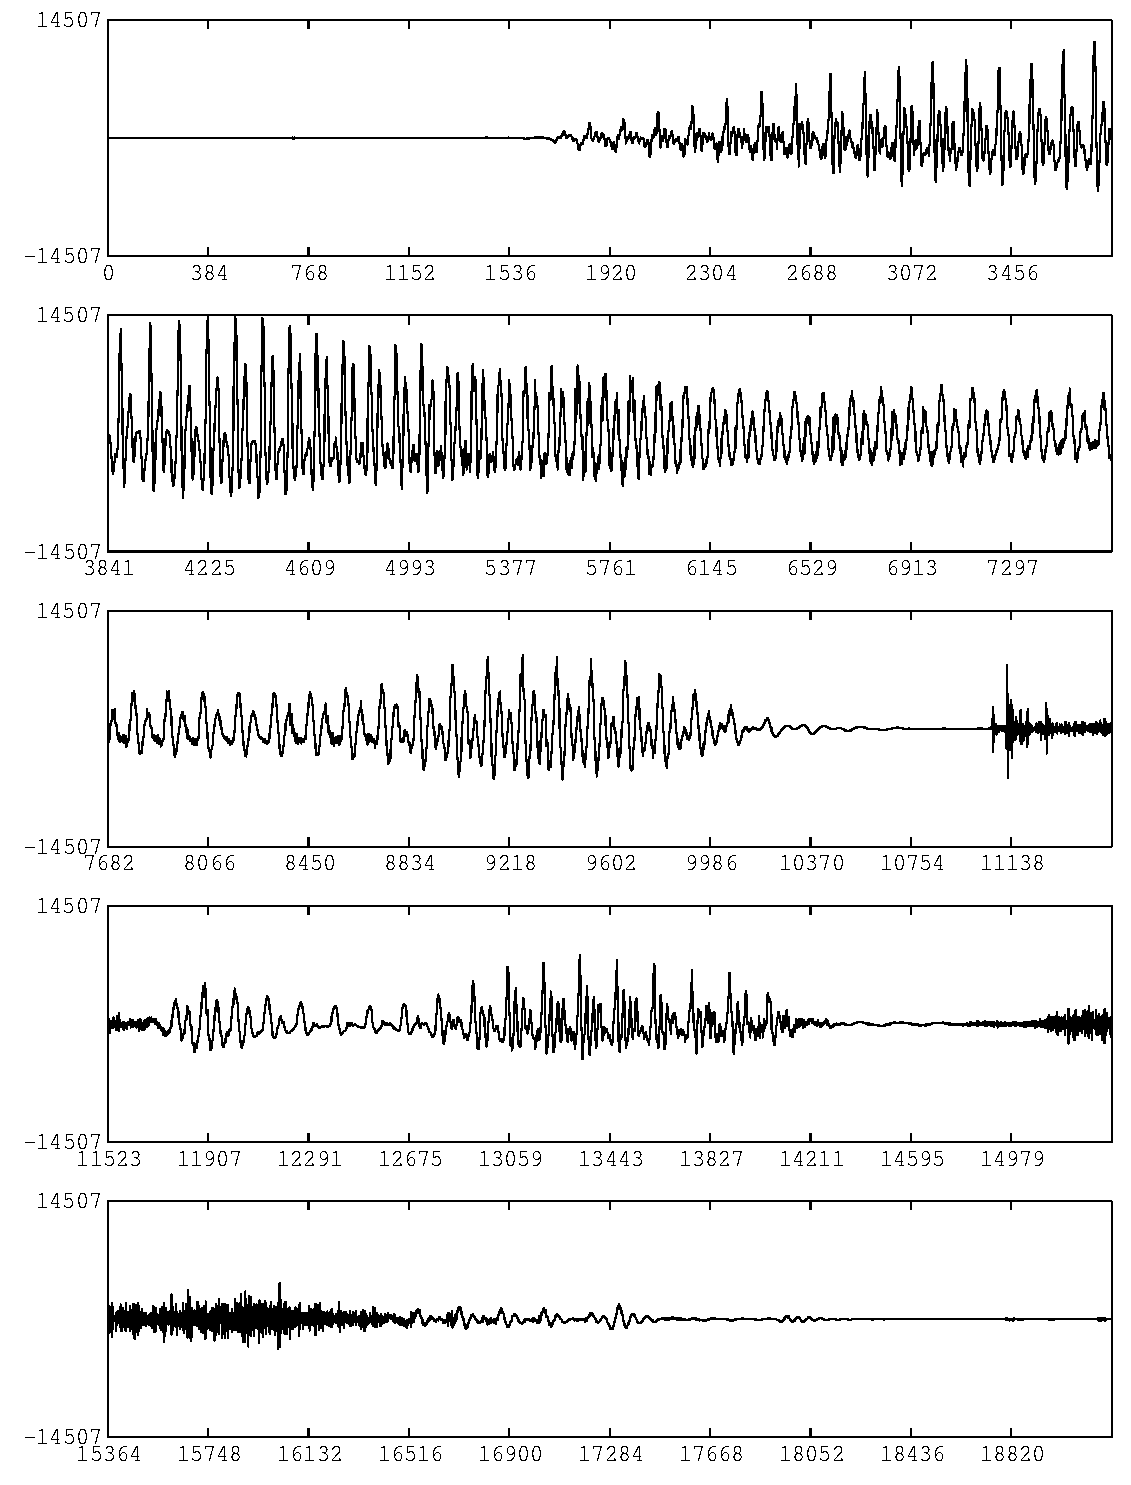
\includegraphics[width=10cm]{eps/data.gwave.eps}

\subsection{Save the figure in an Encapsulated PostScript file}

\begin{description}
\item[Files:]
  data.short: speech data included in this example (short integer, 16 kHz sampling)\\
  figure.eps: Encapsulated PostScript file
\end{description}

\begin{verbatim}
gwave +s data.short | psgr > figure.eps
\end{verbatim}

\subsection{Play a sound file}

\begin{description}
\item[Files:]
  data.short: speech data included in this example (short integer, 16 kHz sampling)
\item[Note:]
  This works only on Linux, Solaris, and FreeBSD.
\end{description}

\begin{verbatim}
da -s 16 -a 100 data.short
\end{verbatim}

\subsection{Cut a portion out of a file}

\begin{description}
\item[Files:]
  data.short: speech data included in this example (short integer, 16 kHz sampling)
\end{description}

\begin{verbatim}
bcut +s -s 1000 -e 11000 < data.short |\
gwave +s | xgr
\end{verbatim}

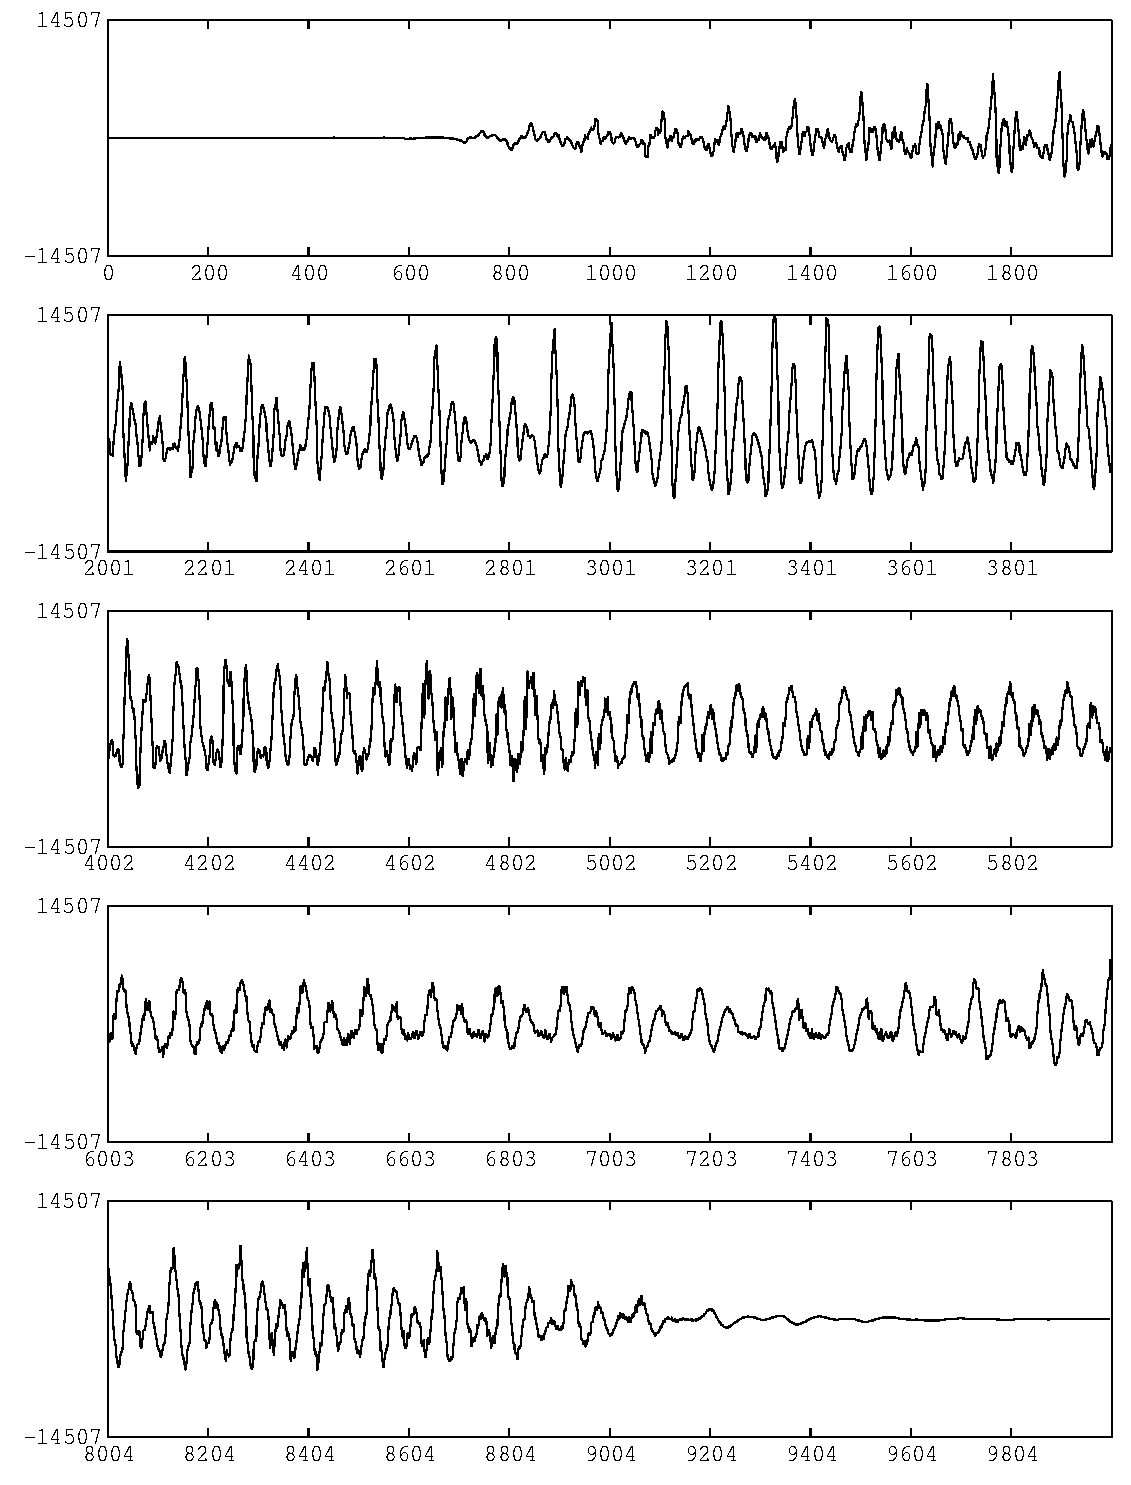
\includegraphics[width=10cm]{eps/data.bcut.gwave.eps}

\section{Pitch Extraction from Speech Waveform}

\subsection{A (very simple) pitch extractor}

\begin{description}
\item[Files:]
  data.short: speech data included in this example (short integer, 16 kHz sampling)\\
\item[Conditions:]
  frame length: 640 points (40 ms)\\
  frame period: 80 points (5 ms)\\
  window: Blackman window
\item[Note:]
  Options should be adjusted for each speech data.
\end{description}

\begin{verbatim}
x2x +sf data.short | frame -l 640 -p 80 |\
window -l 640 | pitch -s 16 -l 640 -t 4.5 -L 60 -H 170 > data.pitch
\end{verbatim}

\subsection{Plotting the extracted pitch contour}

\begin{description}
\item[Files:]
  data.pitch: pitch data extracted from speech data "data.short"
\item[Conditions:]
  Minimum value of vertical axis: 0.0\\
  Maximum value of vertical axis: 250.0\\
  Width: 15 cm\\
  Height: 4 cm
\end{description}

\begin{verbatim}
fdrw -y 0 250 -W 1.5 -H 0.4 < data.pitch | xgr
\end{verbatim}

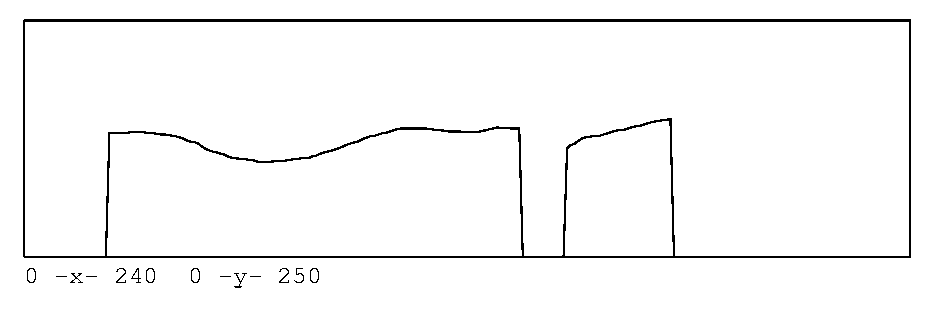
\includegraphics[width=10cm]{eps/data.pitch.fdrw.eps}

\section{Speech Analysis/Synthesis Based on Mel-Cepstral Representation}

\subsection{Mel-cepstral analysis of speech}

\begin{description}
\item[Files:]
  data.short: speech data included in this example (short integer, 16 kHz sampling)\\
  data.mcep: mel-cepstrum (float)
\item[Conditions:]
  frame length: 400 points (25 ms)\\
  frame period: 80 points (5 ms)\\
  window: Blackman window\\
  analysis order: 20\\
  frequency warping parameter: $\alpha = 0.42$\\
  FFT size: 512 points
\end{description}

\begin{verbatim}
x2x +sf < data.short | frame -l 400 -p 80 | window -l 400 -L 512 |\
mcep -l 512 -m 20 -a 0.42 > data.mcep
\end{verbatim}

\subsection{Plotting spectral estimates from mel-cepstrum}

\begin{description}
\item[Files:]
  data.mcep: mel-cepstrum (float)
\item[Conditions:]
  analysis order: 20\\
  frequency warping parameter: $\alpha = 0.42$\\
  FFT size: 512 points\\
  plotted frames: from 10-th to 135-th\\
  sampling frequency: 16 kHz
\end{description}

\begin{verbatim}
bcut -n 20 -s 10 -e 135 < data.mcep |\
mgc2sp -m 20 -a 0.42 -g 0 -l 512 | grlogsp -l 512 -x 8 | xgr
\end{verbatim}

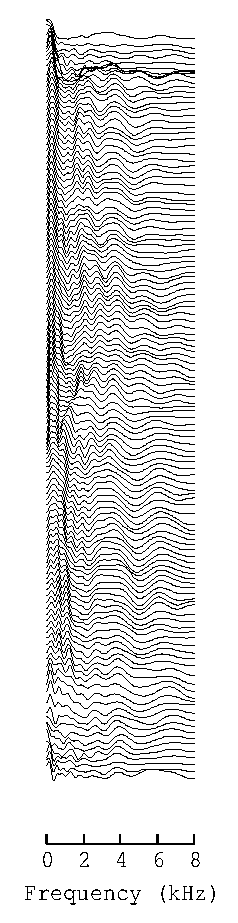
\includegraphics[width=3cm]{eps/data.mcep.grlogsp.eps}

\begin{verbatim}
bcut -n 20 -s 10 -e 135 < data.mcep |\
mgc2sp -m 20 -a 0.42 -g 0 -l 512 | grlogsp -l 512 -x 8 -t | xgr
\end{verbatim}

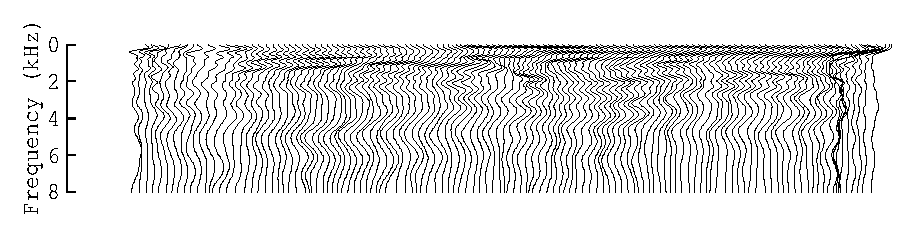
\includegraphics[height=3cm]{eps/data.mcep.grlogsp-t.eps}

\subsection{Plotting the spectral estimate with the FFT spectrum}

\begin{description}
\item[Files:]
  data.mcep: mel-cepstrum (float)
\item[Conditions:]
  analysis order: 20\\
  frequency warping parameter: $\alpha = 0.42$\\
  FFT size: 512 points\\
  plotted frame: 65-th\\
  sampling frequency: 16 kHz
\end{description}

\begin{verbatim}
( x2x +sf < data.short | frame -l 400 -p 80 | \
bcut -l 400 -s 65 -e 65 |\
window -l 400 -L 512 | spec -l 512 |\
glogsp -l 512 -x 8 -p 2 ;\
\
bcut -n 20 -s 65 -e 65 < data.mcep |\
mgc2sp -m 20 -a 0.42 -g 0 -l 512 | glogsp -l 512 -x 8 ) | xgr
\end{verbatim}

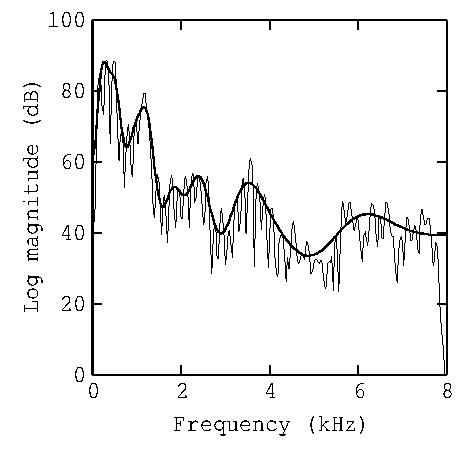
\includegraphics[width=5cm]{eps/data.mcep.glogsp.eps}

\subsection{Speech synthesis from mel-cepstrum}

\begin{description}
\item[Files:]
  data.pitch: pitch data extracted from speech data "data.short"\\
  data.mcep: mel-cepstrum (float) \\
  \includemovie[text={\textcolor[named]{Blue}{\underline{data.mcep.syn}}}]{}{}{wav/data_mcep_syn.wav}: 
  synthesized speech (float)
\item[Conditions:]
  frame period: 80 points (5 ms)\\
  analysis order: 20\\
  frequency warping parameter: $\alpha = 0.42$
\end{description}

\begin{verbatim}
excite -p 80 data.pitch |\
mlsadf -m 20 -a 0.42 -p 80 data.mcep > data.mcep.syn
\end{verbatim}

\begin{verbatim}
gwave data.mcep.syn | xgr
\end{verbatim}

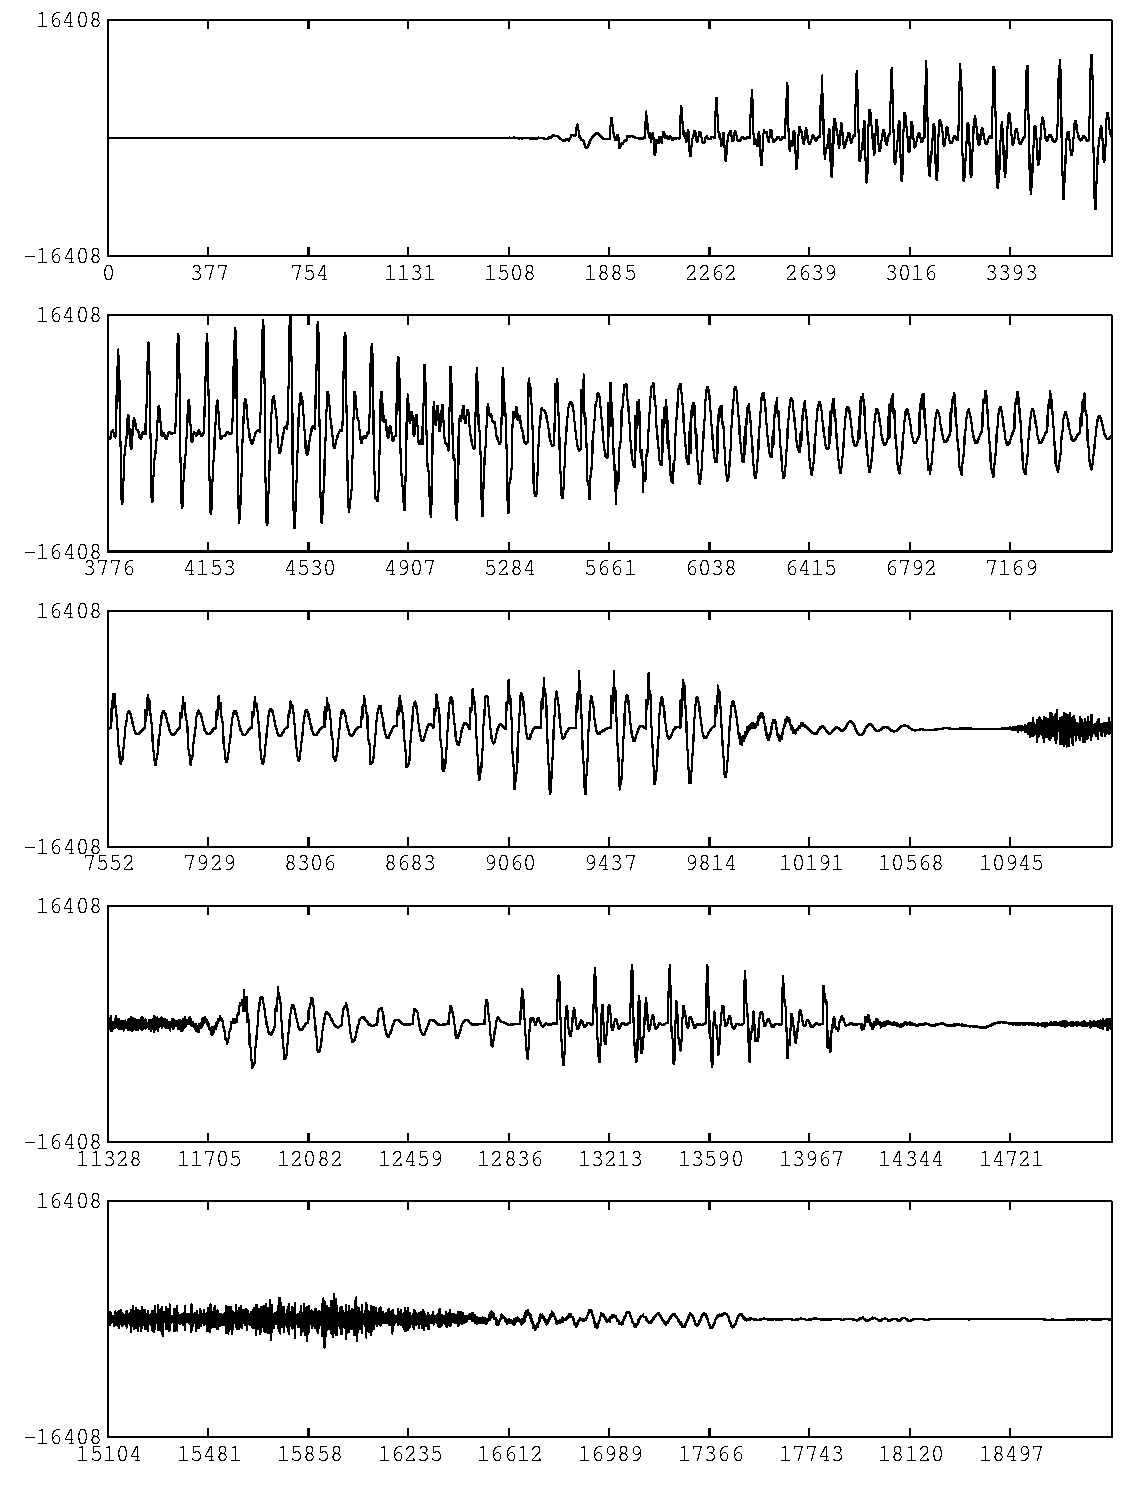
\includegraphics[width=10cm]{eps/data.mcep.syn.gwave.eps}

\begin{verbatim}
da +f -s 16 data.mcep.syn
\end{verbatim}

\section{Speech Analysis/Synthesis based on LPC}

\subsection{LPC analysis of speech}

\begin{description}
\item[Files:]
  data.short: speech data included in this example (short integer, 16 kHz sampling)\\
  data.lpc: LPC coefficients (float)
\item[Conditions:]
  frame length: 400 points (25 ms)\\
  frame period: 80 points (5 ms)\\
  window: Blackman window\\
  analysis order: 20
\end{description}

\begin{verbatim}
x2x +sf < data.short | frame -l 400 -p 80 | window -l 400 |\
lpc -l 400 -m 20 > data.lpc
\end{verbatim}

\subsection{Plotting spectral estimates from LPC coefficients}

\begin{description}
\item[Files:]
  data.lpc: LPC coefficients (float)
\item[Conditions:]
  analysis order: 20
\end{description}

\begin{verbatim}
bcut -n 20 -s 10 -e 135 < data.lpc |\
spec -l 512 -n 20 | grlogsp -l 512 -x 8 | xgr
\end{verbatim}

or

\begin{verbatim}
bcut -n 20 -s 10 -e 135 < data.lpc |\
mgc2sp -m 20 -a 0 -g -1 -n -u -l 512 |\
grlogsp -l 512 -x 8 | xgr
\end{verbatim}

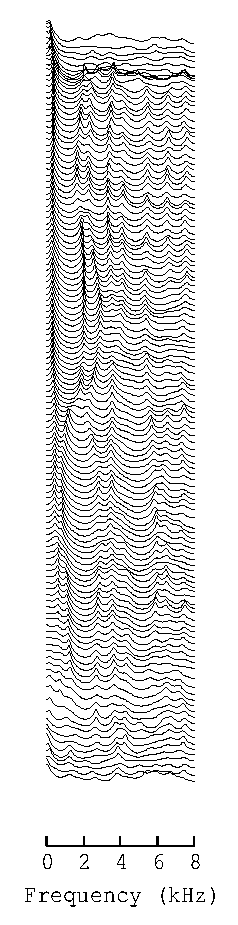
\includegraphics[width=3cm]{eps/data.lpc.grlogsp.eps}

\subsection{Plotting the spectral estimate with the FFT spectrum}

\begin{description}
\item[Files:]
  data.lpc: LPC coefficients (float)
\item[Conditions:]
  analysis order: 20\\
  plotted frame: 65-th\\
  sampling frequency: 16 kHz
\end{description}

\begin{verbatim}
( x2x +sf < data.short | frame -l 400 -p 80 | \
bcut -l 400 -s 65 -e 65 |\
window -l 400 -L 512 | spec -l 512 |\
glogsp -l 512 -x 8 -p 2 ;\
\
bcut -n 20 -s 65 -e 65 < data.lpc > data.tmp ;\
spec -l 512 -n 20 -p data.tmp | glogsp -l 512 -x 8 ;\
\rm data.tmp ) | xgr
\end{verbatim}

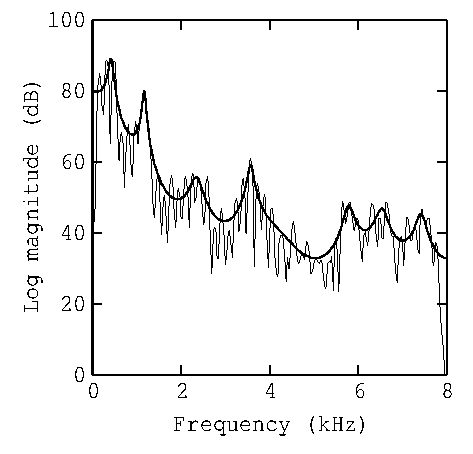
\includegraphics[width=5cm]{eps/data.lpc.glogsp.eps}

\subsection{Speech synthesis from LPC coefficients}

\begin{description}
\item[Files:]
   data.pitch: pitch data extracted from speech data "data"\\
   data.lpc: LPC coefficients (float)\\
\includemovie[text={\textcolor[named]{Blue}{\underline{data.lpc.syn}}}]{}{}{wav/data_lpc_syn.wav}: 
   synthesized speech (float)
\item[Conditions:]
  frame period: 80 points (5 ms)\\
  analysis order: 20
\end{description}

\begin{verbatim}
excite -p 80 data.pitch | poledf -m 20 -p 80 data.lpc > data.lpc.syn
\end{verbatim}

\begin{verbatim}
gwave data.lpc.syn | xgr
\end{verbatim}

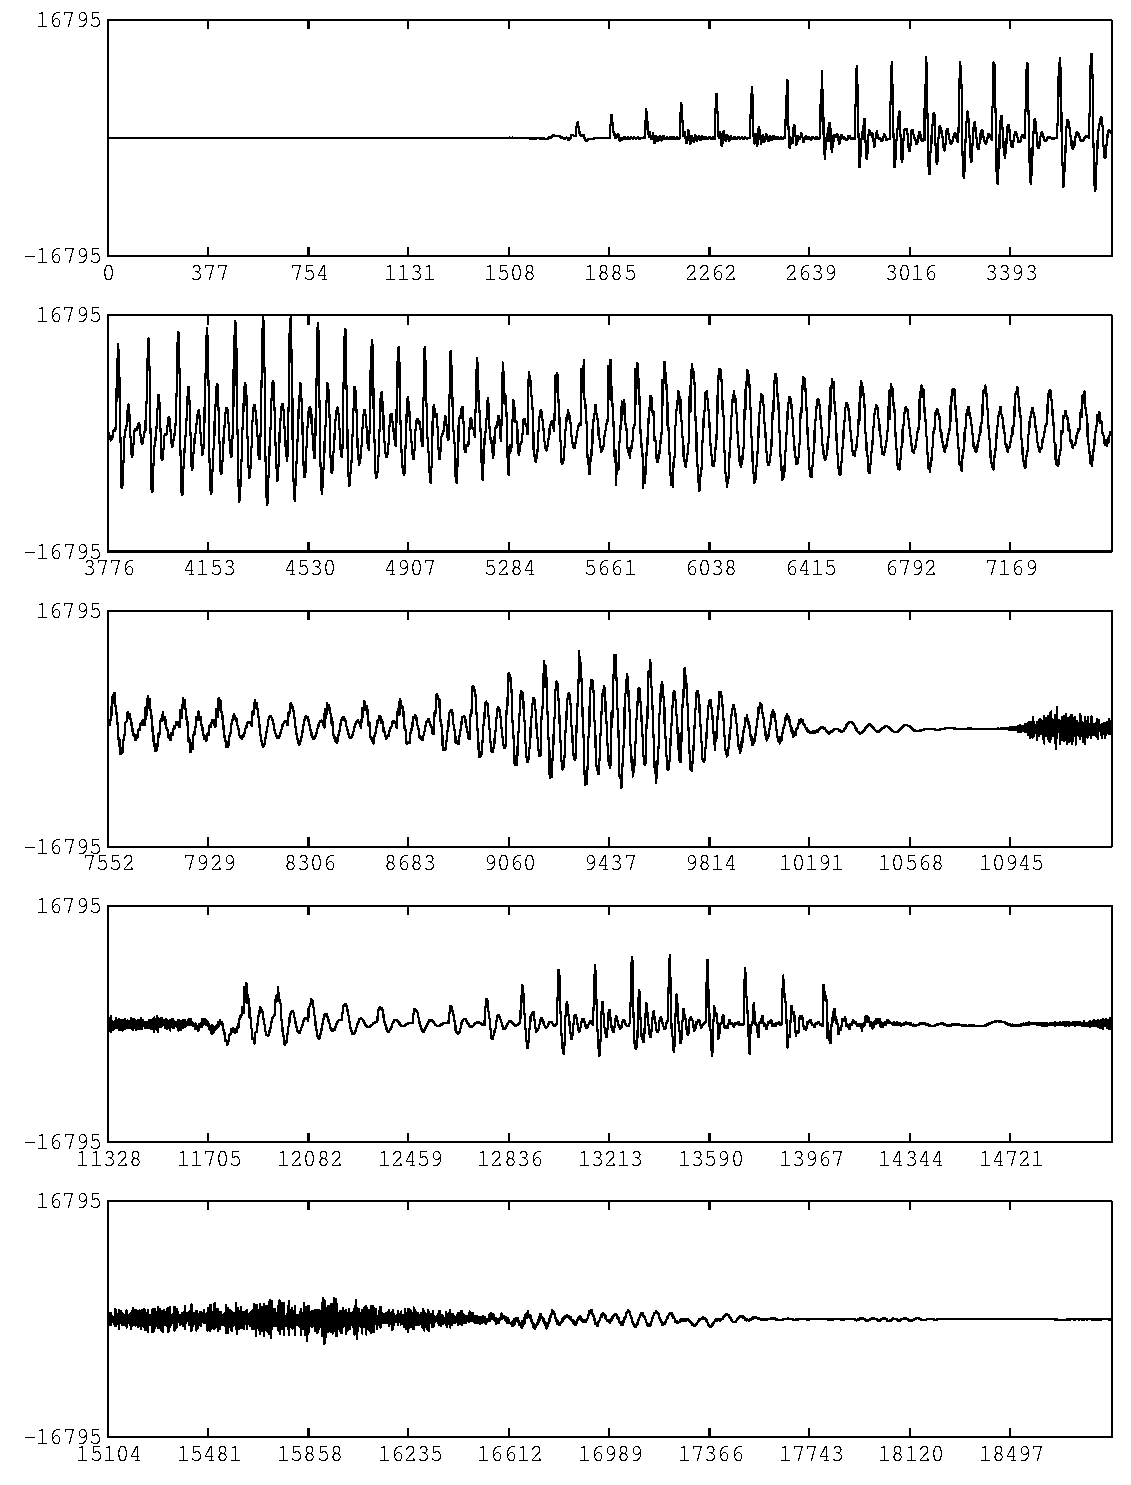
\includegraphics[width=10cm]{eps/data.lpc.syn.gwave.eps}

\begin{verbatim}
da +f -s 16 data.lpc.syn
\end{verbatim}

\subsection{Obtain PARCOR coefficients from LPC coefficients}

\begin{description}
\item[Files:] 
   data.lpc: LPC coefficients (float)\\
   data.par: PARCOR coefficients (float)
\item[Conditions:]
  analysis order: 20
\end{description}

\begin{verbatim}
lpc2par -m 20 < data.lpc > data.par
\end{verbatim}

\subsection{Speech synthesis from PARCOR coefficients}
\begin{description}
\item[Files:]
  data.pitch: pitch data extracted from speech data "data" (float)\\
  data.par: PARCOR coefficients (float)\\
  \includemovie[text={\textcolor[named]{Blue}{\underline{data.par.syn}}}]{}{}{wav/data_par_syn.wav}:
  synthesized speech (float)
\item[Conditions:]
  frame period: 80 points (5 ms)\\
  analysis order: 20
\end{description}

\begin{verbatim}
excite -p 80 data.pitch | ltcdf -m 20 -p 80 data.par > data.par.syn
\end{verbatim}

\begin{verbatim}
gwave data.par.syn | xgr
\end{verbatim}

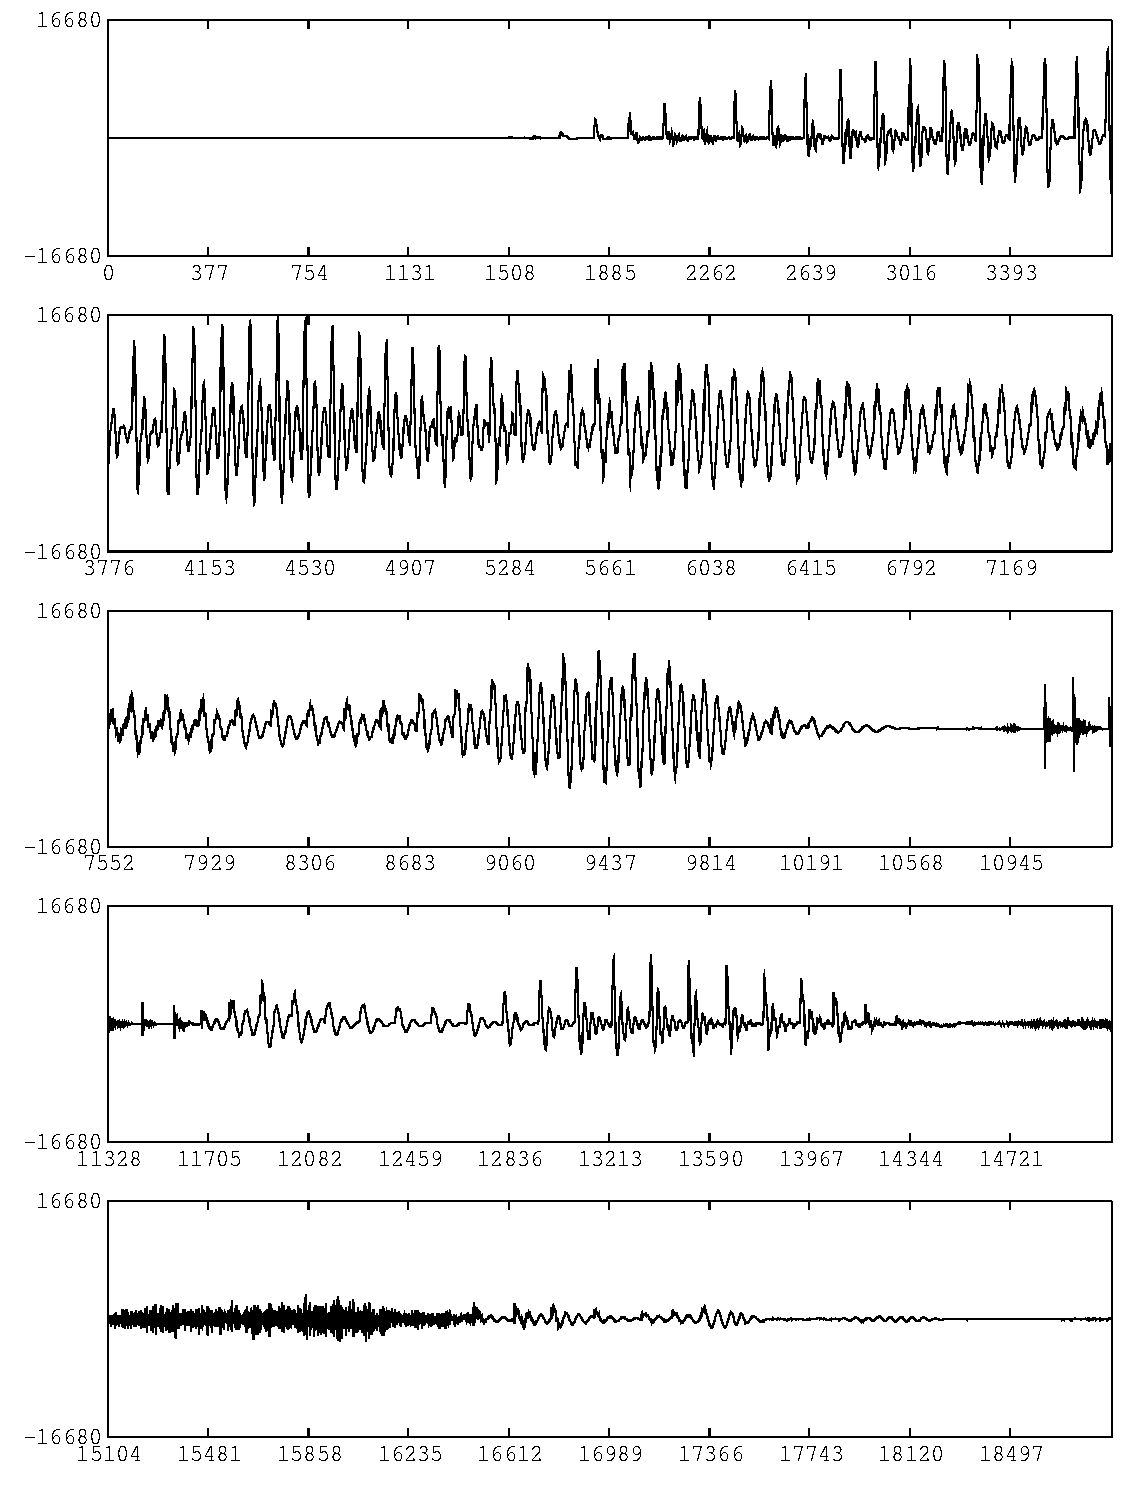
\includegraphics[width=10cm]{eps/data.par.syn.gwave.eps}

\subsection{Obtain LSP coefficients from LPC coefficients}
\begin{description}
\item[Files:]
   data.lpc: LPC coefficients (float)\\
   data.lsp: LSP coefficients (float)
\item[Conditions:]
  analysis order: 20\\
  split number of unit circle: 256
\end{description}

\begin{verbatim}
lpc2lsp -m 20 -n 256 < data.lpc > data.lsp
\end{verbatim}

\subsection{Speech synthesis from LSP coefficients}

\begin{description}
\item[Files:]
  data.pitch: pitch data extracted from speech data "data"\\
  data.lsp: LSP coefficients (float)\\
  \includemovie[text={\textcolor[named]{Blue}{\underline{data.lsp.syn}}}]{}{}{wav/data_lsp_syn.wav}:
  synthesize speech (float)
\item[Conditions:]
  frame period: 80 points (5 ms)\\
  analysis order: 20
\end{description}

\begin{verbatim}
excite -p 80 data.pitch | lspdf -m 20 -p 80 data.lsp > data.lsp.syn
\end{verbatim}

\begin{verbatim}
gwave data.lsp.syn | xgr
\end{verbatim}

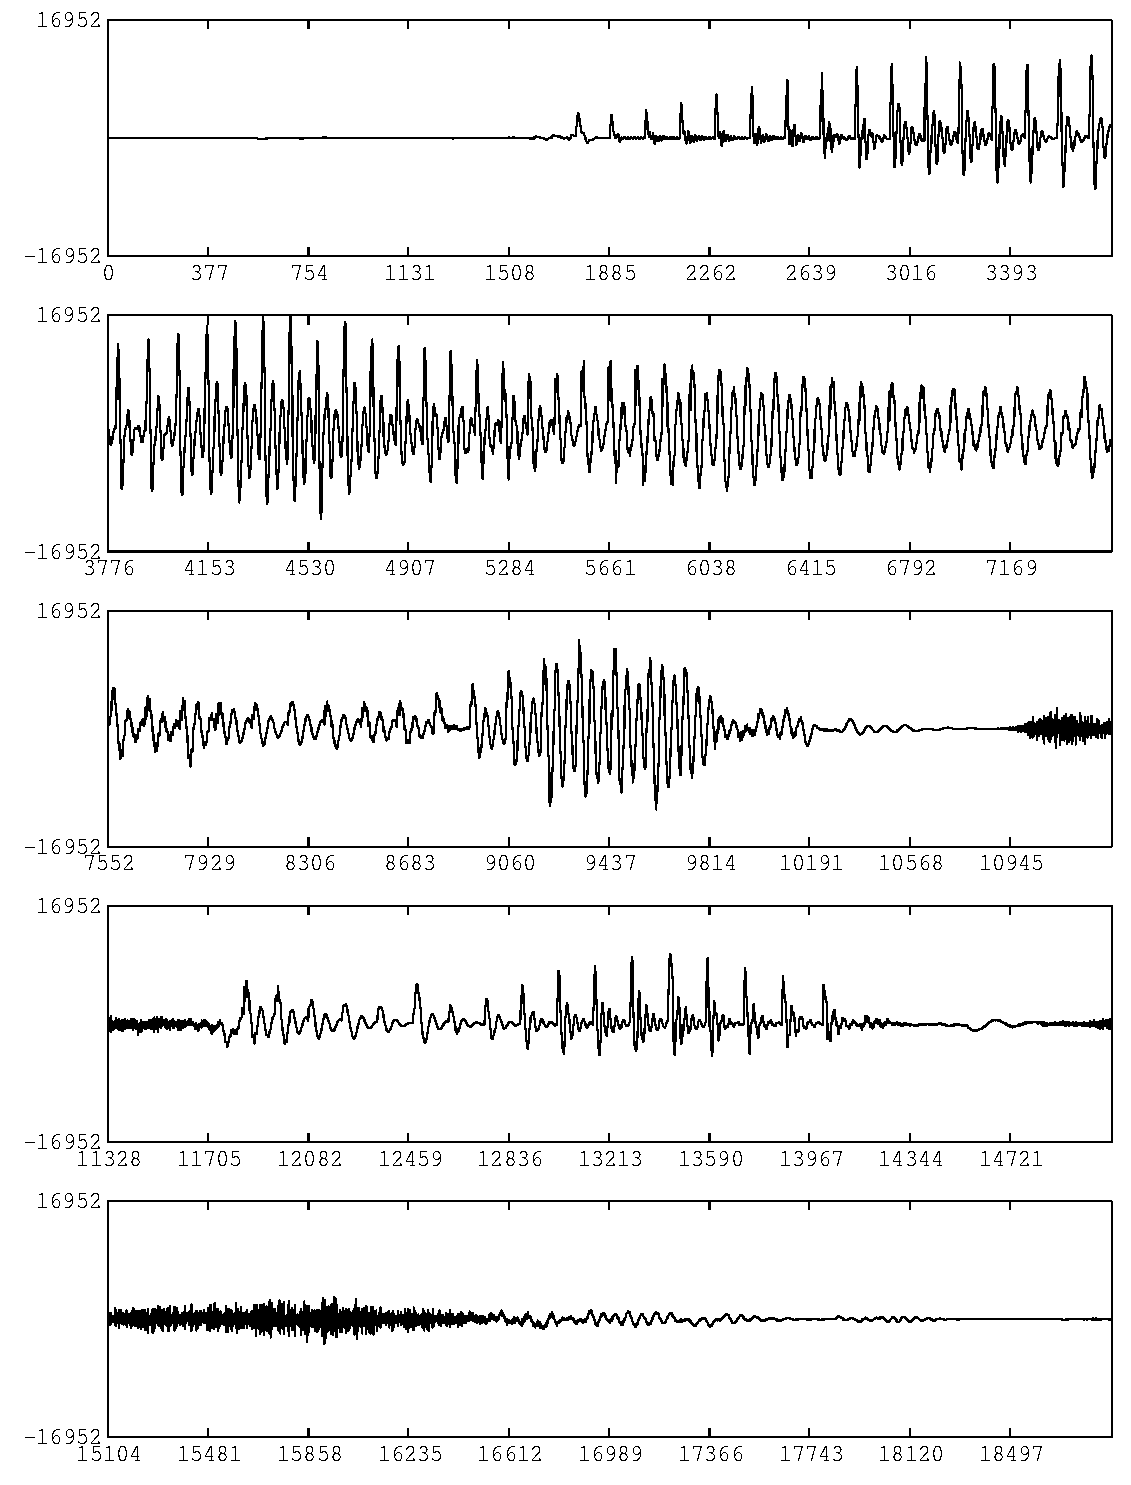
\includegraphics[width=10cm]{eps/data.lsp.syn.gwave.eps}

\begin{verbatim}
da +f -s 16 data.lsp.syn
\end{verbatim}

\section{Speech Analysis/Synthesis 
        Based on Mel-Generalized Cepstral Representation}

\subsection{Mel-generalized cepstral analysis of speech}

\begin{description}
\item[Files:]
   speech data: data (short integer, 10 kHz sampling)\\
   data.mgcep: mel-generalized cepstrum (float)
\item[Conditions:]
  frame length: 400 points (25 ms)\\
  frame period: 80 points (5 ms)\\
  window: Blackman window\\
  analysis order: 20\\
  frequency warping parameter: $\alpha = 0.42$\\
  power parameter:     $\gamma = -1/2$
\end{description}

\begin{verbatim}
x2x +sf < data.short | frame -l 400 -p 80 | window -l 400 -L 512 |\
mgcep -m 20 -a 0.42 -g 2 -l 512 > data.mgcep
\end{verbatim}

\subsection{Plotting spectral estimates from mel-generalized cepstrum}

\begin{description}
\item[Files:]
  data.mgcep: mel-generalize cepstrum (float)
\item[Conditions:]
  analysis order: 20\\
  frequency warping parameter: $\alpha = 0.42$\\
  power parameter: $\gamma = -1/2$\\
  plotted frames: from 10-th to 135-th\\
  sampling frequency: 16 kHz
\end{description}

\begin{verbatim}
bcut -n 20 -s 10 -e 135 < data.mgcep |\
mgc2sp -m 20 -a 0.42 -g 2 -l 512 | grlogsp -l 512 -x 8 | xgr
\end{verbatim}

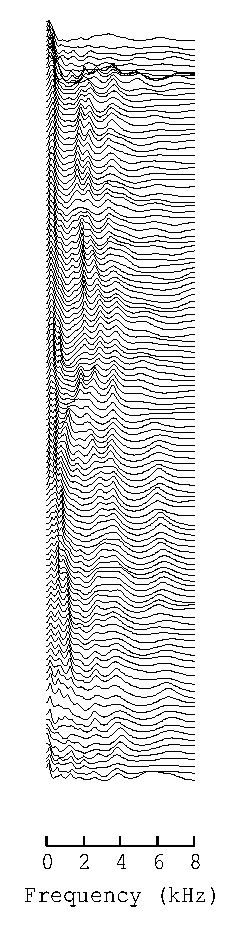
\includegraphics[width=3cm]{eps/data.mgcep.grlogsp.eps}

\subsection{Plotting the spectral estimate with the FFT spectrum}

\begin{description}
\item[Files:]
  data.mgcep: mel-generalized cepstrum (float)
\item[Conditions:]
  analysis order: 20\\
  frequency warping parameter: $\alpha = 0.42$\\
  power parameter: $\gamma = -1/2$\\
  FFT size: 512 points\\
  plotted frame: 65-th\\
  sampling frequency: 16 kHz
\end{description}

\begin{verbatim}
( x2x +sf < data.short | frame -l 400 -p 80 | \
bcut -l 400 -s 65 -e 65 |\
window -l 400 -L 512 | spec -l 512 |\
glogsp -l 512 -x 8 -p 2 ;\
\
bcut -n 20 -s 65 -e 65 < data.mgcep |\
mgc2sp -m 20 -a 0.42 -g 2 -l 512 | glogsp -l 512 -x 8 ) | xgr
\end{verbatim}

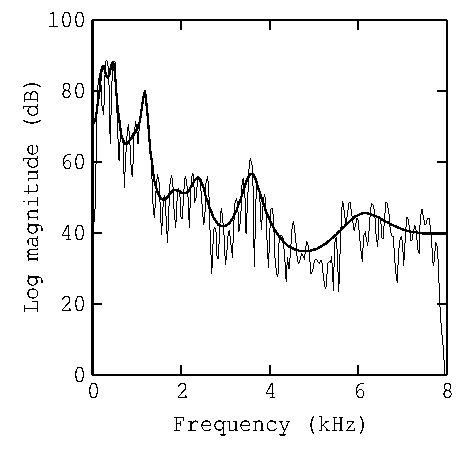
\includegraphics[width=5cm]{eps/data.mgcep.glogsp.eps}

\subsection{Speech synthesis from mel-generalized cepstrum}

\begin{description}
\item[Files:]
  data.pitch: pitch data extracted from speech data "data"\\
  data.mgcep: mel-generalized cepstrum (float)\\
    \includemovie[text={\textcolor[named]{Blue}{\underline{data.mgcep.syn}}}]{}{}{wav/data_mgcep_syn.wav}:
  synthesized speech (float)
\item[Conditions:]
  frame period: 80 points (5 ms)\\
  analysis order: 20\\
  frequency warping parameter: $\alpha = 0.42$\\
  power parameter: $\gamma = -1/2$
\end{description}

\begin{verbatim}
excite -p 80 data.pitch |\
mglsadf -m 20 -a 0.42 -g 2 -p 80 data.mgcep > data.mgcep.syn
\end{verbatim}

\begin{verbatim}
gwave data.mgcep.syn | xgr
\end{verbatim}

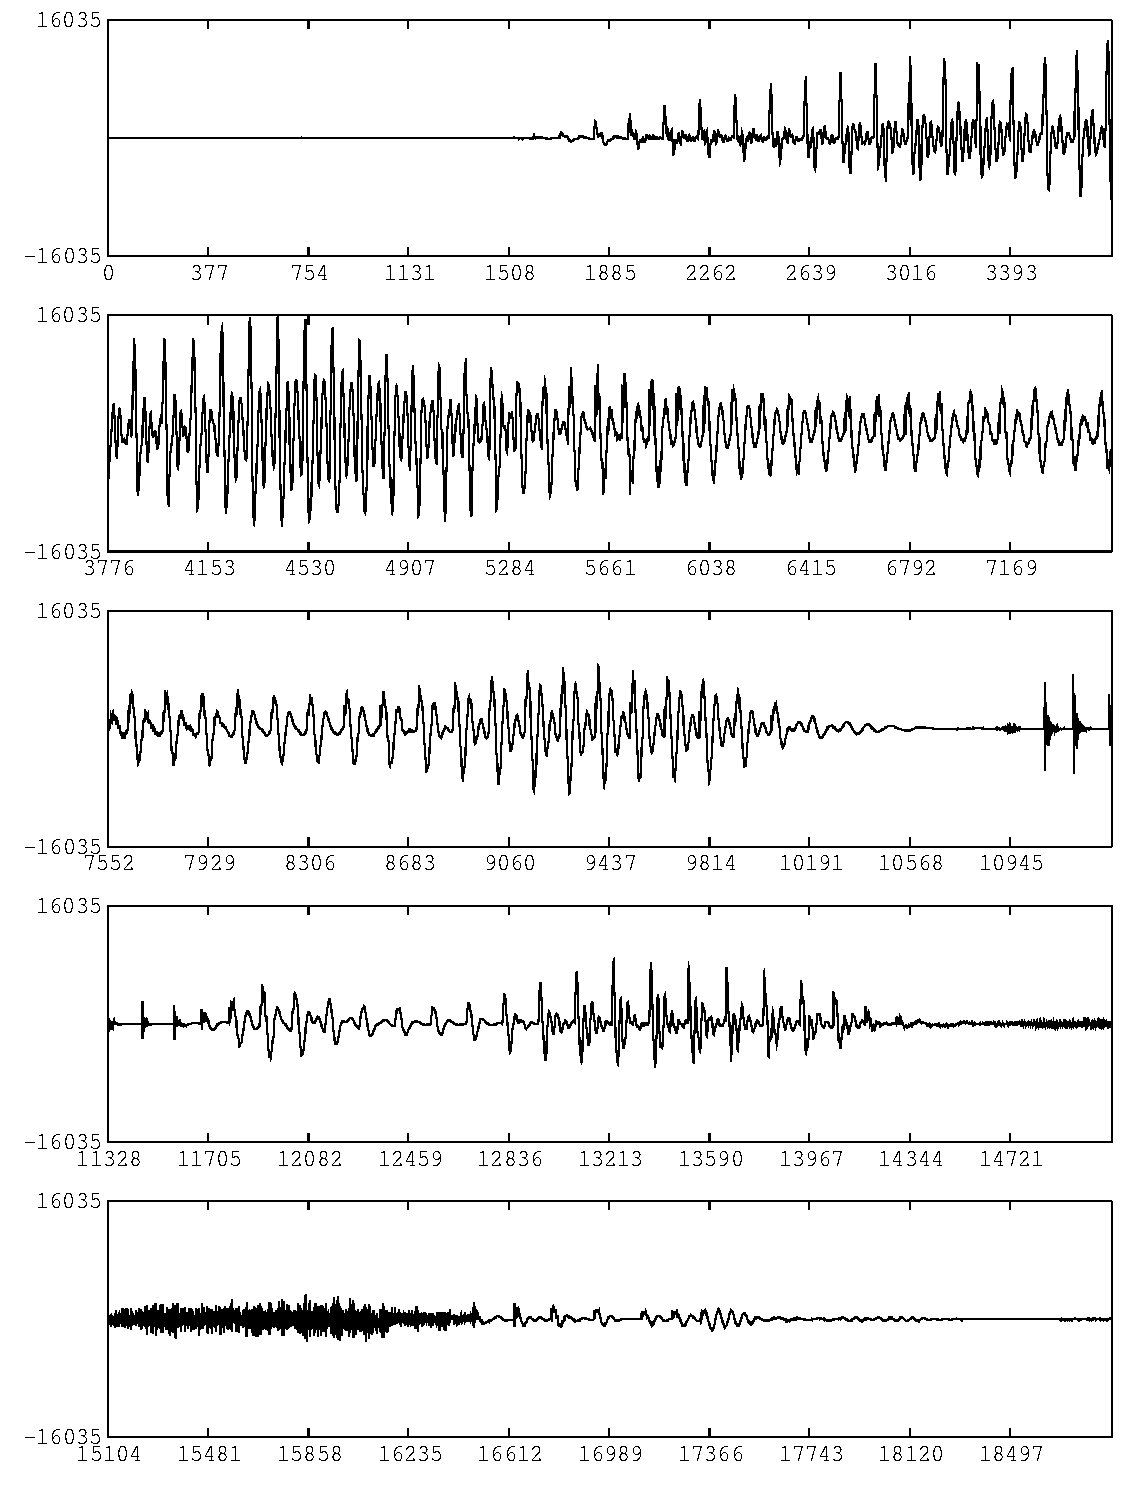
\includegraphics[width=10cm]{eps/data.mgcep.syn.gwave.eps}

\begin{verbatim}
da +f -s 16 data.mgcep.syn
\end{verbatim}

\section{Vector Quantization of Mel-Cepstrum}

\subsection{Train a (very small) Codebook}
\begin{description}
\item[Files:]
   data.mcep: mel-cepstrum for training (float) \\
   codebook.mcep: codebook (float)
\item[Conditions:]
   vector size: 21 (analysis order: 20)\\
   codebook size: 32
\end{description}

\begin{verbatim}
lbg -n 20 -e 32 < data.mcep > codebook.mcep
\end{verbatim}

\subsection{Encode (training vectors)}

\begin{description}
\item[Files:]
   codebook.mcep: codebook (float)\\
   data.mcep.index: index (int)
\item[Conditions:]
   vector size: 21 (analysis order: 20)\\
   codebook size: 32
\end{description}

\begin{verbatim}
vq -n 20 codebook.mcep < data.mcep > data.mcep.index
\end{verbatim}

\subsection{Decode (training vectors)}

\begin{description}
\item[Files:]
   codebook.mcep: codebook (float)\\
   data.mcep.index: index (int)\\
   data.mcep.vq: quantized mel-cepstrum (float)
\item[Conditions:]
   vector size: 21 (analysis order: 20)\\
   codebook size: 32
\end{description}

\begin{verbatim}
ivq -n 20 codebook.mcep < data.mcep.index > data.mcep.vq
\end{verbatim}

\subsection{Plotting original and quantized spectra}

\begin{description}
\item[Files:]
  data.mcep: original mel-cepstrum (float)\\
  data.mcep.vq: quantized mel-cepstrum (float)
\item[Conditions:]
  analysis order: 20\\
  frequency warping parameter: $\alpha = 0.42$\\
  plotted frames: from 10-th to 135-th\\
  sampling frequency: 16 kHz
\end{description}

\begin{verbatim}
( bcut -n 20 -s 10 -e 135 < data.mcep |\
mgc2sp -m 20 -a 0.42 -g 0 -l 512 |\
grlogsp -l 512 -x 8 -O 1 -c "(a) original" ;\
\
bcut -n 20 -s 10 -e 135 < data.mcep.vq |\
mgc2sp -m 20 -a 0.42 -g 0 -l 512 |\
grlogsp -l 512 -x 8 -O 2 -c "(b) quantized" ) | xgr
\end{verbatim}

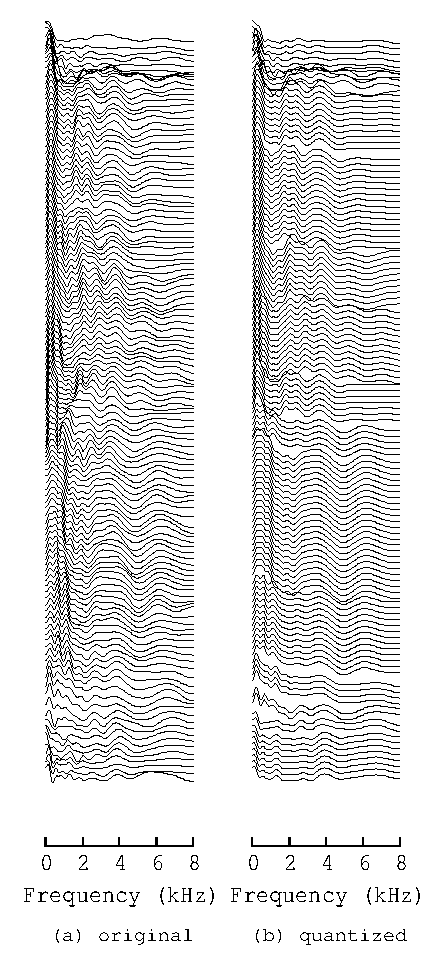
\includegraphics[width=6cm]{eps/data.mcep.vq.grlogsp.eps}

\subsection{Perfomance evaluation on the training data}

\begin{description}
\item[Files:]
   codebook.mcep: codebook (float)\\
   data.mcep.index: index (int)\\
   data.mcep.vq: quantized vectors (float)\\
   data.mcep.vq.cdist: cepstrum distortion in dB (float)
\item[Conditions:]
   vector size: 21 (analysis order: 20)\\
   codebook size: 32
\end{description}

\begin{verbatim}
freqt -a 0.42 -m 20 -A 0 -M 255 < data.mcep > data.mcep.cep
freqt -a 0.42 -m 20 -A 0 -M 255 < data.mcep.vq |\
cdist data.mcep.cep -m 255 > data.mcep.vq.cdist
\rm data.mcep.cep
\end{verbatim}

\subsection{Speech synthesis from quantized mel-cepstrum}

\begin{description}
\item[Files:]
  data.pitch: pitch data extracted from speech data "data.short"\\
  data.mcep.vq: quantized mel-cepstrum (float) \\
  \includemovie[text={\textcolor[named]{Blue}{\underline{data.mcep.vq.syn}}}]{}{}{wav/data_mcep_vq_syn.wav}:
  synthesized speech (float)
\item[Conditions:]
  frame period: 80 points (5 ms)\\
  analysis order: 20 \\
  frequency warping parameter: $\alpha = 0.42$
\end{description}

\begin{verbatim}
excite -p 80 data.pitch |\
mlsadf -m 20 -a 0.42 -p 80 data.mcep.vq > data.mcep.vq.syn
\end{verbatim}

\begin{verbatim}
gwave data.mcep.vq.syn | xgr
\end{verbatim}

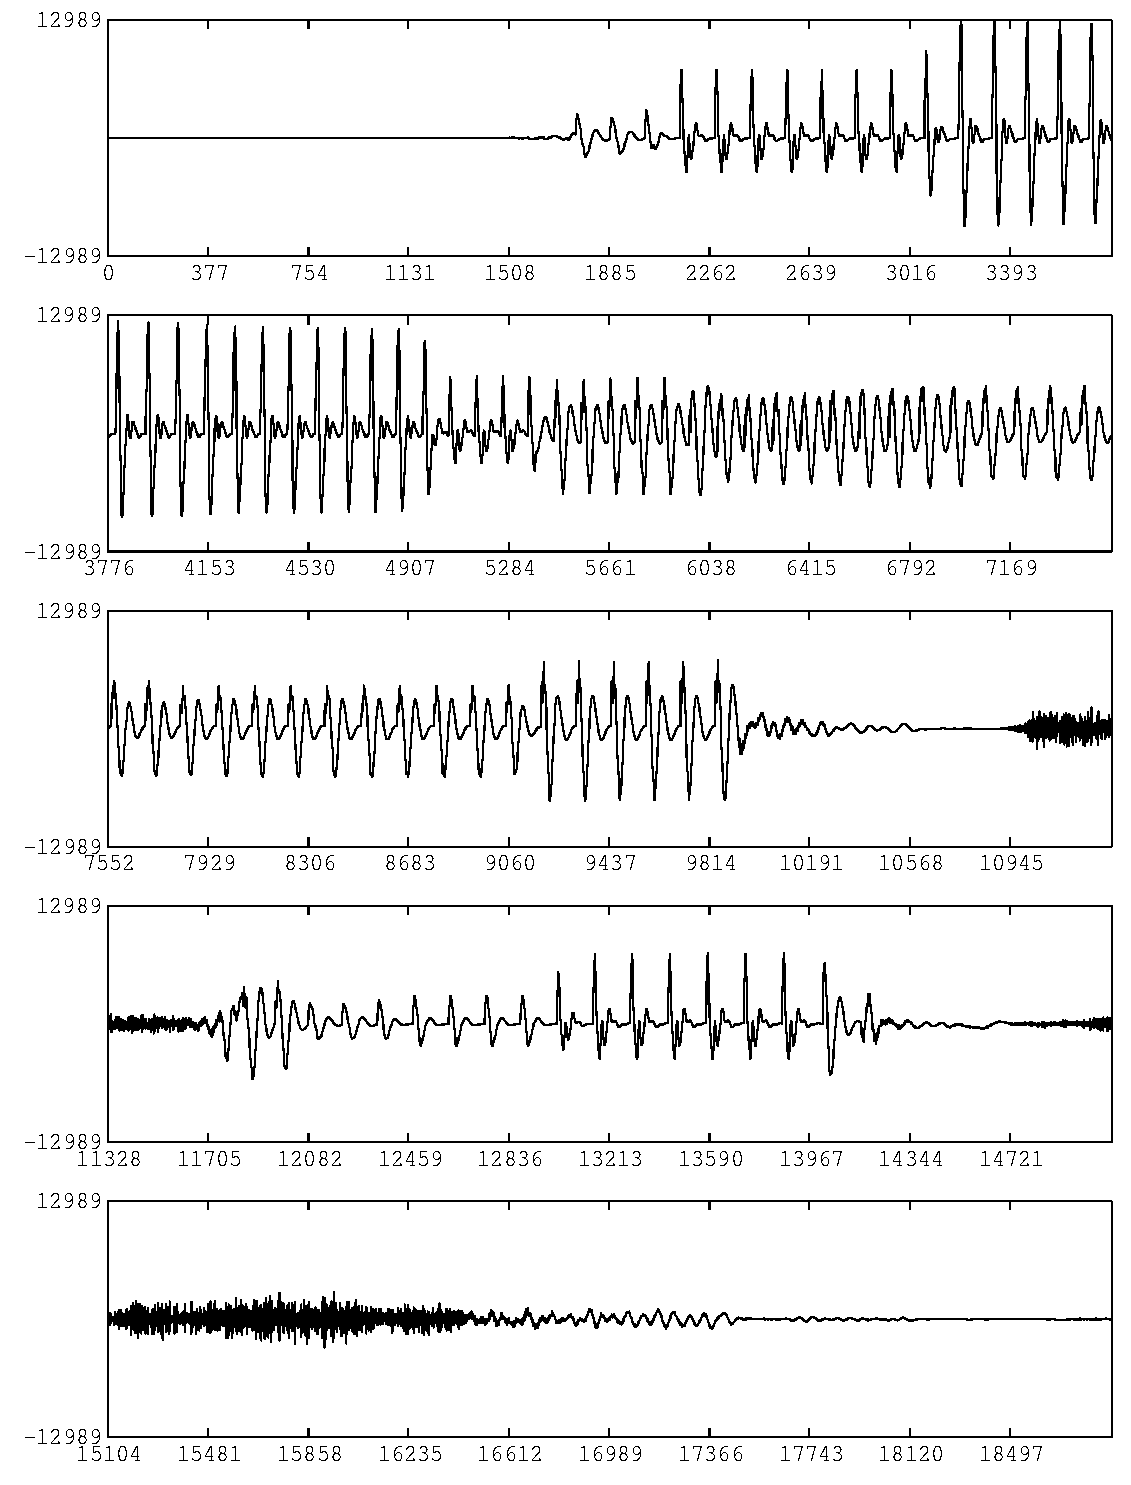
\includegraphics[width=10cm]{eps/data.mcep.vq.syn.gwave.eps}

\begin{verbatim}
da +f -s 16 data.mcep.vq.syn
\end{verbatim}

\section{Preparation of Speech Parameter for Speech Recognition}

\subsection{Cepstrum derived from LPC analysis (LPC cepstrum)}

\begin{description}
\item[Files:] 
  data.short: speech data included in this example (short integer, 16 kHz sampling)
\item[Conditions:]
  frame length: 400 points (25 ms)\\
  frame period: 80 points (5 ms)\\
  window: Blackman window\\
  analysis order: 12\\
  order of LPC cepstrum: 12
\end{description}

\begin{verbatim}
x2x +sf < data.short | frame -l 400 -p 80 | window -l 400 |\
lpc -l 400 -m 12 | lpc2c -m 12 -M 12 > data.lpc.cep
\end{verbatim}

\subsection{Mel-cepstrum derived from LPC analysis
  (LPC mel-cepstrum)}

\begin{description}
\item[Files:]
  data.short: speech data included in this example (short integer, 16 kHz sampling)
\item[Conditions:]
  frame length: 400 points (25 ms)\\
  frame period: 80 points (5 ms)\\
  window: Blackman window\\
  analysis order: 12\\
  order of LPC mel-cepstrum: 12
\end{description}

\begin{verbatim}
x2x +sf < data.short | frame -l 400 -p 80 | window -l 400 |\
lpc -l 400 -m 12 |\
lpc2c -m 12 -M 256 |\
freqt -m 256 -a 0 -M 12 -A 0.42 > data.lpc.mcep
\end{verbatim}

or

\begin{verbatim}
x2x +sf < data.short | frame -l 400 -p 80 | window -l 400 |\
lpc -l 400 -m 12 |\
mgc2mgc -m 12 -a 0 -g -1 -n -u -M 12 -A 0.42 -G 0 > data.lpc.mcep
\end{verbatim}

\subsection{Mel-cepstrum obtained by mel-cepstral analysis}

\begin{description}
\item[Files:]
  data.short: speech data included in this example (short integer, 16 kHz sampling)\\
  data.mcep: mel-cepstrum (float)
\item[Conditions:]
  frame length: 400 points (25 ms)\\
  frame period: 80 points (5 ms)\\
  window: Blackman window\\
  analysis order: 20 \\
  frequency warping parameter: $\alpha = 0.42$\\
  FFT size: 512 points
\end{description}

\begin{verbatim}
x2x +sf < data.short | frame -l 400 -p 80 | window -l 400 -L 512 |\
mcep -l 512 -m 12 -a 0.42 > data.mcep.mcep
\end{verbatim}

\subsection{Mel-cepstrum derived from mel-generalized cepstral analysis}

\begin{description}
\item[Files:]
   data.short: speech data included in this example (short integer, 10 kHz sampling)\\
\item[Conditions:]
  frame length: 400 points (25 ms)\\
  frame period: 80 points (5 ms)\\
  Blackman window\\
  FFT size: 512 points\\
  $(\alpha, \gamma)$ for analysis: (0.42, -0.5)\\
  analysis order: 12\\
  order of mel-cepstrum: 12
\end{description}

\begin{verbatim}
x2x +sf < data.short | frame -l 400 -p 80 | window -l 400 -L 512 |\
mgcep -m 12 -a 0.42 -g 2 -l 512 |\
mgc2mgc -m 12 -a 0.42 -g 2 -M 12 -A 0.42 -G 0 > data.mgcep.mcep
\end{verbatim}

\subsection{Plotting spectra for each speech recognition parameter}

\begin{description}
\item[Files:]
  data.lpc.cep: LPC cepstrum (float)\\
  data.lpc.mcep: LPC mel-cepstrum (float)\\
  data.mcep.mcep: mel-cepstrum  (float)\\
  data.mgcep.mcep: mel-cepstrum derived from mel-generalized cepstrum (float)
\item[Conditions:]
  plotted frames: from 10-th to 135-th\\
\end{description}

\begin{verbatim}
(\
bcut -n 12 -s 10 -e 135 < data.lpc.cep |\
mgc2sp -m 12 -a 0 -g 0 -l 512 |\
grlogsp -l 512 -x 8 -O 1 -c "(a) LPC-CEP" ;\
\
bcut -n 12 -s 10 -e 135 < data.lpc.mcep |\
mgc2sp -m 12 -a 0.42 -g 0 -l 512 |\
grlogsp -l 512 -x 8 -O 2 -c "(b) LPC-MCEP" ;\
\
bcut -n 12 -s 10 -e 135 < data.mcep.mcep |\
mgc2sp -m 12 -a 0.42 -g 0 -l 512 |\
grlogsp -l 512 -x 8 -O 3 -c "(c) MCEP" ;\
\
bcut -n 12 -s 10 -e 135 < data.mgcep.mcep |\
mgc2sp -m 12 -a 0.42 -g 0 -l 512 |\
grlogsp -l 512 -x 8 -O 4 -c "(d) MGCEP-MCEP" ) | xgr
\end{verbatim}

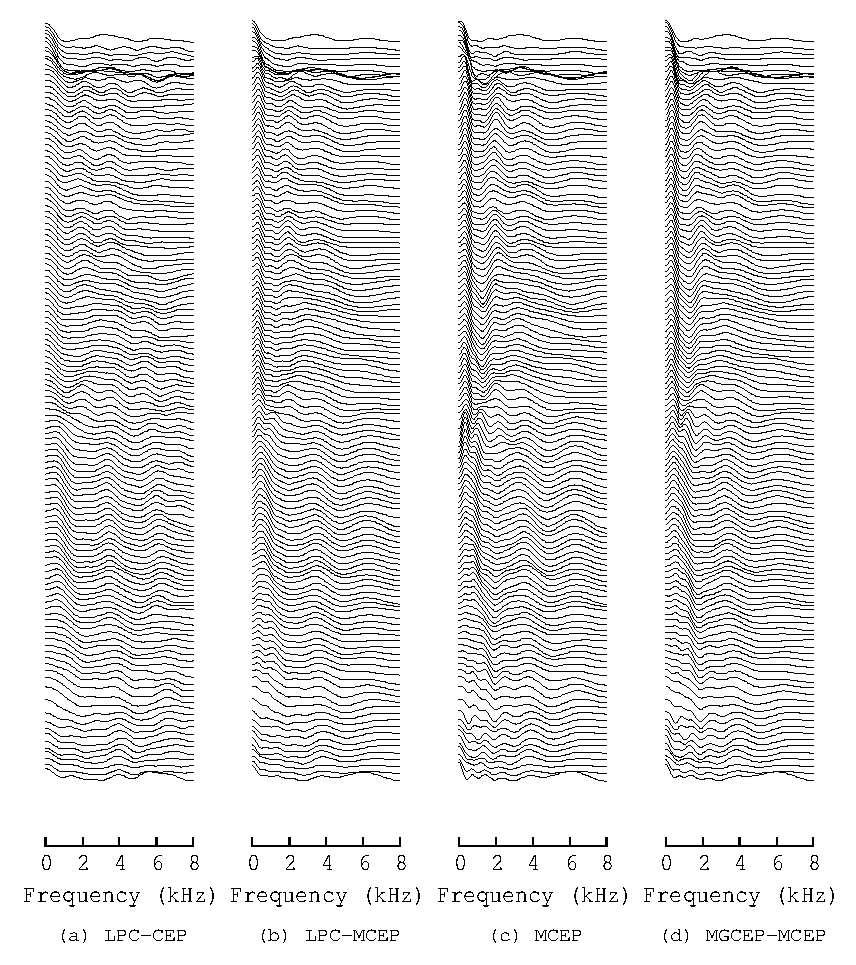
\includegraphics[width=12cm]{eps/data.all.mcep.grlogsp.eps}

\section{Playing with the Vocoder Based on Mel-Cepstrum}

\subsection{High- or low-pitched voice}

\begin{description}
\item[Files:]
  \includemovie[text={\textcolor[named]{Blue}{\underline{data.mcep.high.syn}}}]{}{}{wav/data_mcep_high_syn.wav}:
  synthesized speech (float)\\
  \includemovie[text={\textcolor[named]{Blue}{\underline{data.mcep.low.syn}}}]{}{}{wav/data_mcep_low_syn.wav}:
  synthesized speech (float)
\end{description}

\begin{verbatim}
sopr -m 0.4 data.pitch |\
excite -p 80 | mlsadf -m 20 -a 0.42 -p 80 data.mcep |\
tee data.mcep.high.syn | da +f -s 16
\end{verbatim}

\begin{verbatim}
sopr -m 2 data.pitch |\
excite -p 80 | mlsadf -m 20 -a 0.42 -p 80 data.mcep |\
tee data.mcep.low.syn | da +f -s 16
\end{verbatim}

\subsection{Fast- or slow-speaking voice}

\begin{description}
\item[Files:]
  \includemovie[text={\textcolor[named]{Blue}{\underline{data.mcep.fast.syn}}}]{}{}{wav/data_mcep_fast_syn.wav}:
  synthesized speech (float)\\
  \includemovie[text={\textcolor[named]{Blue}{\underline{data.mcep.slow.syn}}}]{}{}{wav/data_mcep_slow_syn.wav}:
  synthesized speech (float)
\end{description}

\begin{verbatim}
sopr -m 1 data.pitch |\
excite -p 40 | mlsadf -m 20 -a 0.42 -p 40 data.mcep |\
tee data.mcep.fast.syn | da +f -s 16
\end{verbatim}

\begin{verbatim}
sopr -m 1 data.pitch |\
excite -p 160 | mlsadf -m 20 -a 0.42 -p 160 data.mcep |\
tee data.mcep.slow.syn | da +f -s 16
\end{verbatim}

\subsection{Hoarse voice}

\begin{description}
\item[Files:]
  \includemovie[text={\textcolor[named]{Blue}{\underline{data.mcep.hoarse.syn}}}]{}{}{wav/data_mcep_hoarse_syn.wav}:
  synthesized speech (float)\\
\end{description}

\begin{verbatim}
sopr -m 0 data.pitch |\
excite -p 80 | mlsadf -m 20 -a 0.42 -p 80 data.mcep |\
tee data.mcep.hoarse.syn | da +f -s 16 
\end{verbatim}

\subsection{Robotic voice}

\begin{description}
\item[Files:]
  \includemovie[text={\textcolor[named]{Blue}{\underline{data.mcep.robot.syn}}}]{}{}{wav/data_mcep_robot_syn.wav}:
  synthesized speech (float)
\end{description}

\begin{verbatim}
train -p 200 -l -1 | mlsadf -m 20 -a 0.42 -p 80 data.mcep |\
tee data.mcep.robot.syn | da +f -s 16
\end{verbatim}

\subsection{Child-like or deep voice}

\begin{description}
\item[Files:]
  \includemovie[text={\textcolor[named]{Blue}{\underline{data.mcep.child.syn}}}]{}{}{wav/data_mcep_child_syn.wav}:
  synthesized speech (float)\\
  \includemovie[text={\textcolor[named]{Blue}{\underline{data.mcep.deep.syn}}}]{}{}{wav/data_mcep_deep_syn.wav}:
  synthesized speech (float)
\end{description}

\begin{verbatim}
sopr -m 0.4 data.pitch |\
excite -p 80 | mlsadf -m 20 -a 0.1 -p 80 data.mcep |\
tee data.mcep.child.syn | da +f -s 16
\end{verbatim}

\begin{verbatim}
sopr -m 2 data.pitch |\
excite -p 80 | mlsadf -m 20 -a 0.6 -p 80 data.mcep |\
tee data.mcep.deep.syn | da +f -s 16
\end{verbatim}

\subsection{Various voices}

\begin{description}
\item[Files:]
  \includemovie[text={\textcolor[named]{Blue}{\underline{data.float}}}]{}{}{wav/data_float.wav}:
  original speech (float)\\
  \includemovie[text={\textcolor[named]{Blue}{\underline{data.mcep.syn}}}]{}{}{wav/data_mcep_syn.wav}:
  synthesized speech (float)\\
  data.mcep.\{
  \includemovie[text={\textcolor[named]{Blue}{\underline{high}}}]{}{}{wav/data_mcep_high_syn.wav},
  \includemovie[text={\textcolor[named]{Blue}{\underline{low}}}]{}{}{wav/data_mcep_low_syn.wav},
  \includemovie[text={\textcolor[named]{Blue}{\underline{fast}}}]{}{}{wav/data_mcep_fast_syn.wav},
  \includemovie[text={\textcolor[named]{Blue}{\underline{slow}}}]{}{}{wav/data_mcep_slow_syn.wav},
  \includemovie[text={\textcolor[named]{Blue}{\underline{hoarse}}}]{}{}{wav/data_mcep_hoarse_syn.wav},
  \includemovie[text={\textcolor[named]{Blue}{\underline{robot}}}]{}{}{wav/data_mcep_robot_syn.wav},
  \includemovie[text={\textcolor[named]{Blue}{\underline{child}}}]{}{}{wav/data_mcep_child_syn.wav},
  \includemovie[text={\textcolor[named]{Blue}{\underline{deep}}}]{}{}{wav/data_mcep_deep_syn.wav}
  \}.syn: 
  synthesized speech (float)
\end{description}

\begin{verbatim}
da -v +f -s 16 data.float data.mcep.syn \
data.mcep.{high,low,fast,slow,hoarse,robot,child,deep}.syn
\end{verbatim}

\section{Speech Synthesis Based on HMM}

\subsection{Speech parameter generation from a sequence of HMMs}

\begin{description}
\item[Files:]
  sample.pdf: sequence of mean and variance
              corresponding to a state sequence included in this example (float, little endian)\\
  sample.mcep: mel-cepstrum generated from a sequence of HMMs (float)
\item[Conditions:]
  analysis order: 24\\
  weight coefficients for calculating delta: $w(-1)=-0.5,w(0)=0,w(1)=0.5$\\
  weight coefficients for calculating delta-delta: $w(-1)=0.25,w(0)=-0.5,w(1)=0.25$
\item[Note:]
  The state sequence is determined according to the state
  duration densities of the HMMs.  The algorithm is not included
  in SPTK-3.1.
\end{description}

\begin{verbatim}
mlpg -m 24 -d -0.5 0 0.5 -d 0.25 -0.5 0.25 sample.pdf > sample.mcep
\end{verbatim}

\subsection{Plotting spectra calculated from generated mel-cepstrum}

\begin{description}
\item[Files:]
  sample.mcep: mel-cepstral coefficients (float)
\item[Conditions:]
  analysis order: 24\\
  frequency warping parameter: $\alpha = 0.42$\\
  FFT size: 512 points\\
  plotted frames: from 100-th to 250-th\\
  sampling frequency: 16 kHz
\end{description}

\begin{verbatim}
bcut -n 24 -s 100 -e 250 < sample.mcep |\
mgc2sp -m 24 -a 0.42 -g 0 -l 512 | grlogsp -l 512 -x 8 -t | xgr
\end{verbatim}

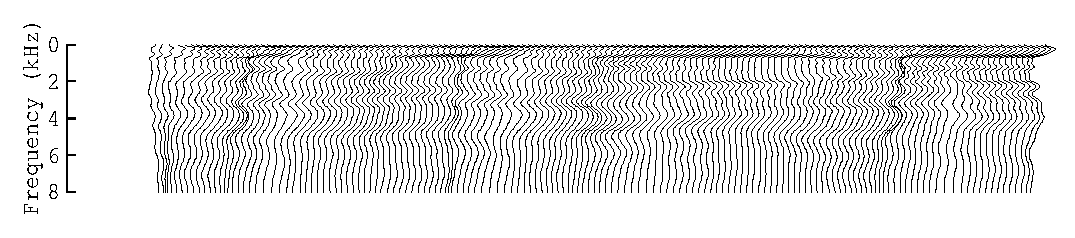
\includegraphics[height=3cm]{eps/sample.mcep.grlogsp-t.eps}

\subsection{Speech synthesis from the generated mel-cepstrum}

\begin{description}
\item[Files:]
  sample.pitch: pitch data generated from a sequence of MSD-HMMs included in this
  example (float, little endian)\\
  sample.mcep: mel-cepstrum (float) \\
  \includemovie[text={\textcolor[named]{Blue}{\underline{sample.mcep.syn}}}]{}{}{wav/sample_mcep_syn.wav}:
  synthesized speech (float)
\item[Conditions:]
  frame period: 80 points (5 ms)\\
  analysis order: 24\\
  frequency warping parameter: $\alpha = 0.42$
\item[Note:]
  The pitch pattern generation algorithm is not included in SPTK-3.1.
\end{description}

\begin{verbatim}
excite -p 80 sample.pitch |\
mlsadf -p 80 -a 0.42 -m 24 sample.mcep > sample.mcep.syn
\end{verbatim}

\begin{verbatim}
gwave +f sample.mcep.syn | xgr
\end{verbatim}

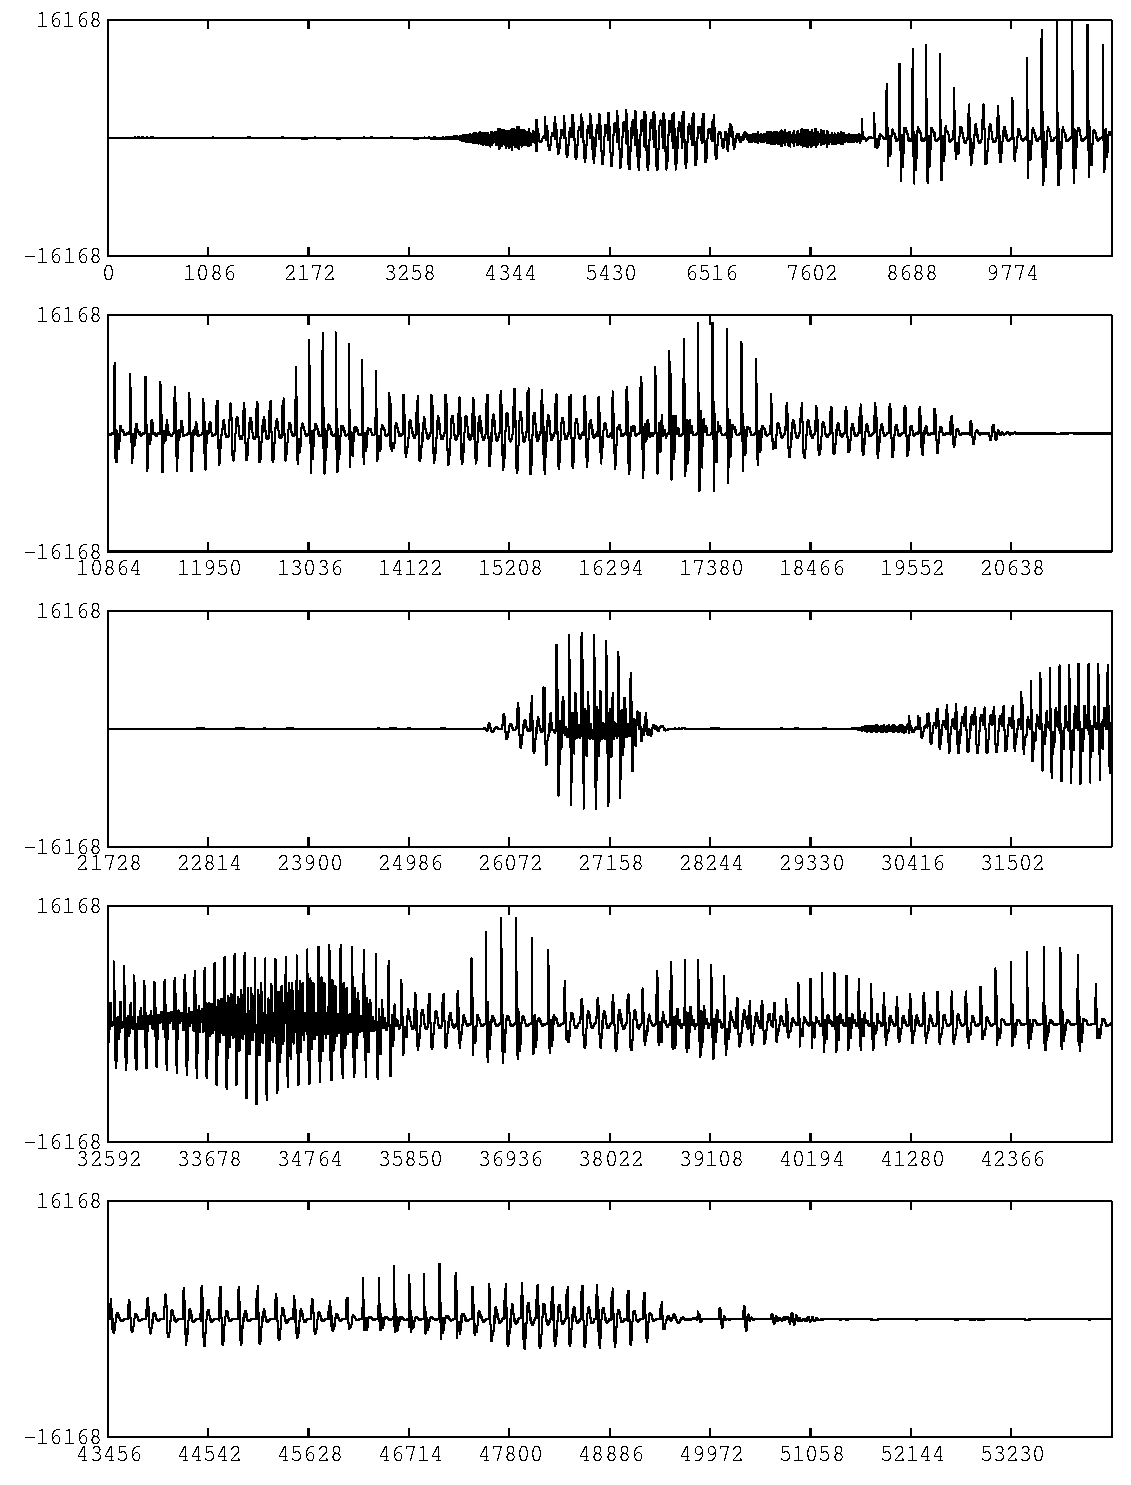
\includegraphics[width=10cm]{eps/sample.mcep.syn.gwave.eps}

\begin{verbatim}
da +f -s 16 sample.mcep.syn
\end{verbatim}

\subsection{Check the given mean and variance vectors}

\begin{description}
\item[Files:]
  sample.pdf: sequence of mean and variance
              corresponding to a state sequence (float)
\item[Conditions:]
  analysis order: 24
\end{description}

\subsubsection{Dump static feature vectors}

\begin{verbatim}
bcp -l 150 -s 0 -e 24 sample.pdf | dmp -n 24 | less
\end{verbatim}

\subsubsection{Dump variance vectors of static feature vectors}

\begin{verbatim}
bcp -l 150 -s 75 -e 99 sample.pdf | dmp -n 24 | less
\end{verbatim}

\subsubsection{Dump dynamic feature vectors (delta)}

\begin{verbatim}
bcp -l 150 -s 25 -e 49 sample.pdf | dmp -n 24 | less
\end{verbatim}

\subsubsection{Dump variance vectors of dynamic feature vectors (delta)}

\begin{verbatim}
bcp -l 150 -s 100 -e 124 sample.pdf | dmp -n 24 | less
\end{verbatim}

\subsection{Speech synthesis without dynamic feature}

\begin{description}
\item[Files:]
  sample.pitch: pitch data generated from a sequence of MSD-HMMs (float)\\
  sample.mcep.wo-dyn: mel-cepstrum generated without dynamic
  feature (float) \\
  \includemovie[text={\textcolor[named]{Blue}{\underline{sample.mcep.wo-dyn.syn}}}]{}{}{wav/sample_mcep_wo-dyn_syn.wav}:
  synthesized speech without dynamic feature (float)
\item[Conditions:]
  frame period: 80 points (5 ms)\\
  analysis order: 24\\
  frequency warping parameter: $\alpha = 0.42$
\end{description}

\begin{verbatim}
bcp -l 150 -s 0 -e 24 sample.pdf > sample.mcep.wo-dyn
\end{verbatim}

\begin{verbatim}
bcut -n 24 -s 100 -e 250 < sample.mcep.wo-dyn |\
mgc2sp -m 24 -a 0.42 -g 0 -l 512 | grlogsp -l 512 -x 8 -t | xgr
\end{verbatim}

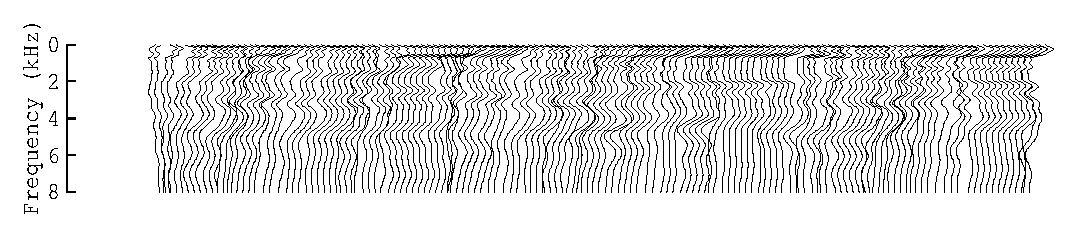
\includegraphics[height=3cm]{eps/sample.mcep.wo-dyn.grlogsp-t.eps}

\begin{verbatim}
excite -p 80 sample.pitch |\
mlsadf -p 80 -a 0.42 -m 24 sample.mcep.wo-dyn > sample.mcep.wo-dyn.syn
\end{verbatim}

\begin{verbatim}
gwave +f sample.mcep.wo-dyn.syn | xgr
\end{verbatim}

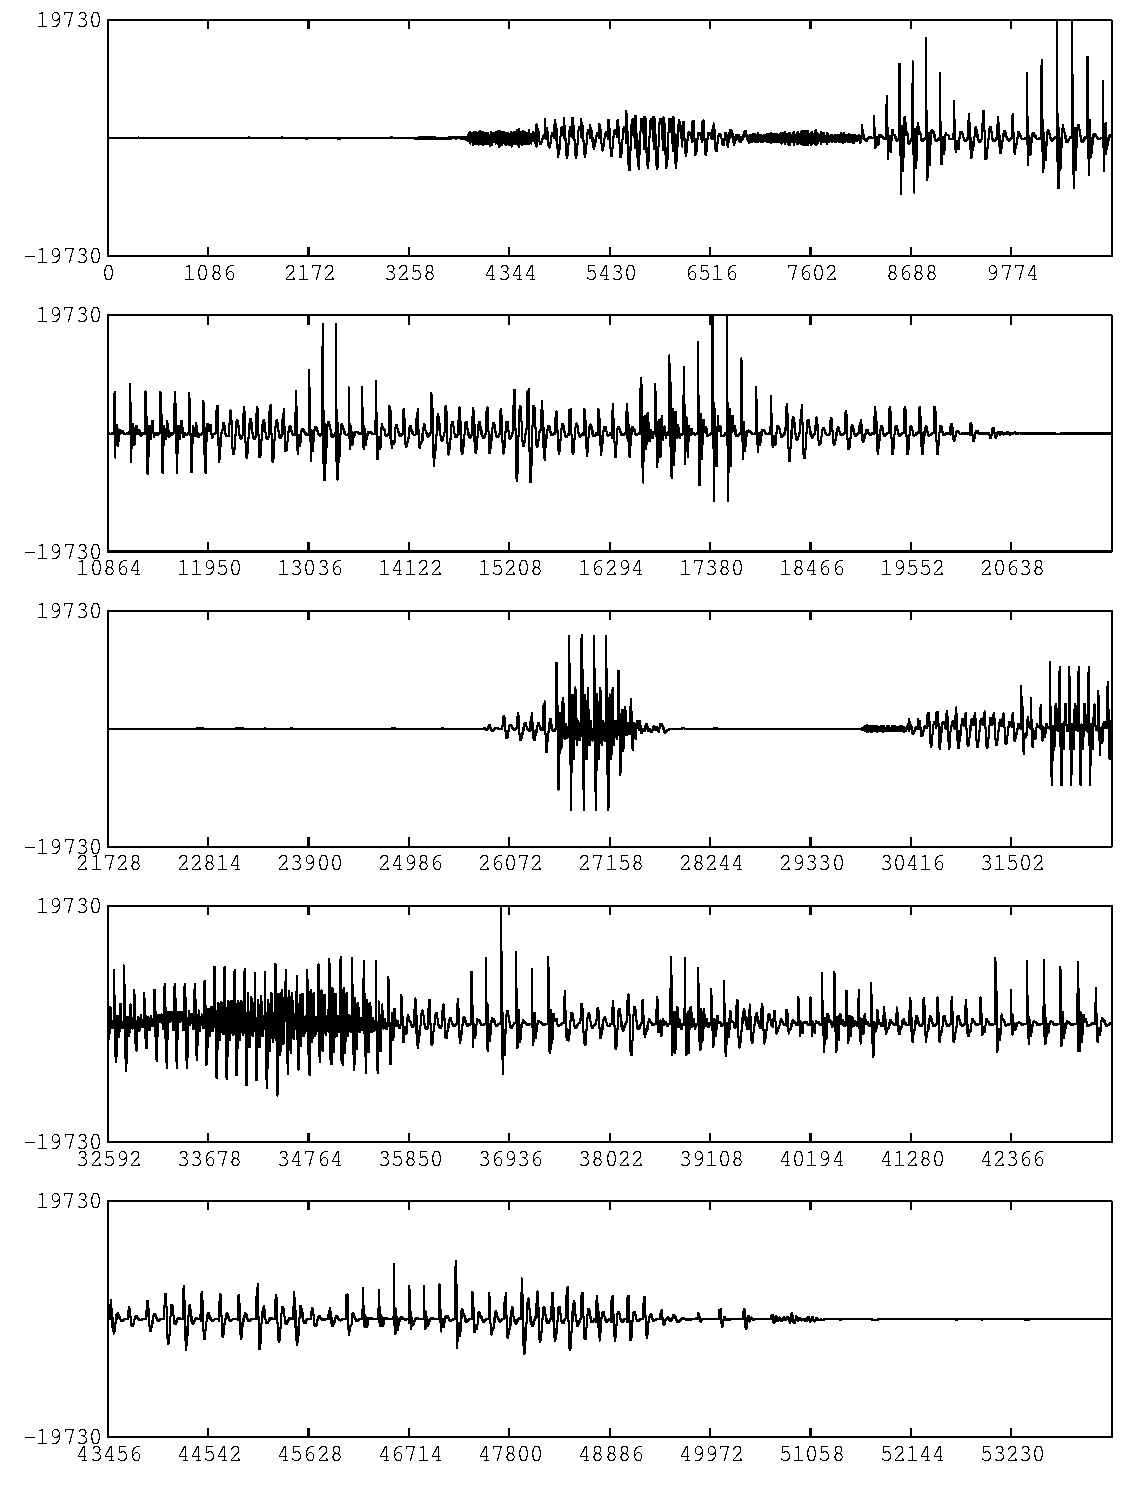
\includegraphics[width=10cm]{eps/sample.mcep.wo-dyn.syn.gwave.eps}

\begin{verbatim}
da +f -s 16 sample.mcep.wo-dyn.syn sample.mcep.syn
\end{verbatim}

\end{document}
